\documentclass{layout/tudelft-aiaa}

%% Additional packages
\usepackage[T1]{fontenc}
\usepackage[utf8]{inputenc}

\usepackage{graphicx} % Adding images
\usepackage{amsmath,amssymb} % Mathematics, symbols
\usepackage{siunitx} % Various functions, e.g. \num{}
\usepackage{tabularx} % Additional functions to tables
\usepackage{subcaption} % Subfigures and subcaptions

%% Additional commands
\setlength{\nomitemsep}{-\parsep} % Reduce white space in nomenclature
\setlength{\bibsep}{1pt} % Reduce white space in references
\renewcommand{\deg}{\si{\degree}\xspace}

%%%%% Title %%%%%

\title{Scientific Article Template for AE2223-I}

\author{List of Authors}
\affil{Project Group Affiliation}

\begin{document}

\AlwaysPagewidth{

\maketitle

%%%%% Abstract %%%%%

\begin{abstract}
    \noindent  The abstract should appear at the beginning of your paper and it should not exceed 250 words. It should be one paragraph long and it should be comprehensible on its own, separately from the rest of the article. It should concisely indicate the background, scientific gap, research question or purpose, method, main results and conclusions dealt with in the article. Do not cite references in the abstract. The abstract is bold and indented 3 picas (1/2”) on each side by default.
\end{abstract}

}

%%%%% Nomenclature %%%%%

\renewcommand{\nompreamble}{\emph{Use this section to provide a list of all symbols used in the report. Provide a concise description. For example:}} %

\printnomenclature[\nomwidest]

\nomenclature{A}{amplitude of oscillation}
\nomenclature{Cp}{pressure coefficient}
\nomenclature{Cx}{force coefficient in the x direction}
\nomenclature{Cy}{force coefficient in the y direction}
\nomenclature{c}{chord}
\nomenclature{dt}{time step}
\nomenclature{Fx}{X component of the resultant pressure force acting on the vehicle}
\nomenclature{Fy}{Y component of the resultant pressure force acting on the vehicle}
\nomenclature{f, g}{generic functions}
\nomenclature{h}{height}
\nomenclature{i}{time index during navigation}

%%%%% Main Body %%%%%

\section{Introduction}

\lettrine{T}{his} template is a simple article template following all the guidelines of AE2333-I, based on the official AIAA template. Refer to the AE2333-I Word template to see all the procedures and guidelines. Please note that you are free to use other formatting styles, as long as you are consistent in how you apply them throughout your text. By default, the article is in one column. Switching to two columns can be done using the \emph{twocolumn} global option, resulting in the following first line in article.tex: \emph{\textbackslash documentclass[twocolumn]\{layout/tudelft-aiaa\}}.


\section{Methodology}

Below, some detailed instruction regarding the typsetting can be found. These instructions are based on the official AIAA template and follow the guidelines of AE2223-I.

\subsection{Document Text}
The default font for your report is Times New Roman, 11-point size. The first line of every paragraph should be indented, with the exception of paragraphs that follow a heading or a blank line (in case of the latter, use \verb+\noindent+). All lines should be single-spaced. Default margins are 1” on all sides. In the electronic version of this template, all margins and other formatting is preset. Limit the use of abbreviations such as e.g. or viz.

\subsection{Headings}
The title of your paper should be typed in bold, 18-point type, with capital and lower-case letters, and centered at the top of the page. The names of the authors and the affiliation should follow on separate lines below the title. Author names are centered, and affiliations are centered and in italic type.

\begin{itemize}
    \item Major headings (\verb+\sections{}+) are bold 11-point font, centered, and numbered with Roman numerals.
    \item Subheadings (\verb+\subsections{}+) are bold, flush left, and numbered with capital letters.
    \item Sub-subheadings (\verb+\subsubsections{}+) are italic, flush left, and numbered (1. 2. 3. etc.)
\end{itemize}

\subsection{In-text References}
Choose and output style that you will use for your references and apply this style consistently throughout your paper. Make sure that you know what your in text references should look like and how different publication types (e.g. books, journal papers etc.) should  be formatted in the reference list.  Examples of references styles are:

\begin{itemize}
    \item AIAA, in which the references are numbered following the order of appearance in your text (for examples of titles in the Reference list, see the “References” section on page 4 of this template. For documentation, see articlee.bib), and
    \item APA, in which you present the name(s) of the author(s) and the year of publication in your text and references are sorted alphabetically in the reference list.
\end{itemize}

\subsection{Footnotes}
Footnotes, where they appear, should be placed above the 1” margin at the bottom of the page. To insert footnotes into the template, use \verb+\footnote{}+. Superscript numbers for footnotes are used by default. Use footnotes scarcely and only to provide additional information that is not essential to understand your argumentation in the main text.

\subsection{Images, Figures, and Tables}
Captions are bold and justified, with a period and a single tab (no hyphen or other character) between the figure number and figure description.

Place figure captions below all figures; place table titles over the tables. If your figure has multiple parts, include the labels “a),” “b),” etc. below and to the left of each part, above the figure caption. Please verify that the figures and tables you mention in the text actually exist. When citing a figure in the text, use the abbreviation “Fig.” except at the beginning of a sentence. Do not abbreviate “Table.” Number each different type of illustration (i.e., figures, tables) sequentially with relation to other illustrations of the same type.

Figure axis labels are often a source of confusion. Use words rather than symbols. As in the example below (\autoref{fig:sample}), write the quantity “Magnetization” rather than just “M.” Do not label axes with units only.
Figure labels must be legible, approximately 8-12 point type. Only use colors for your illustrations if needed.

\begin{figure}[htb]
    \centering
    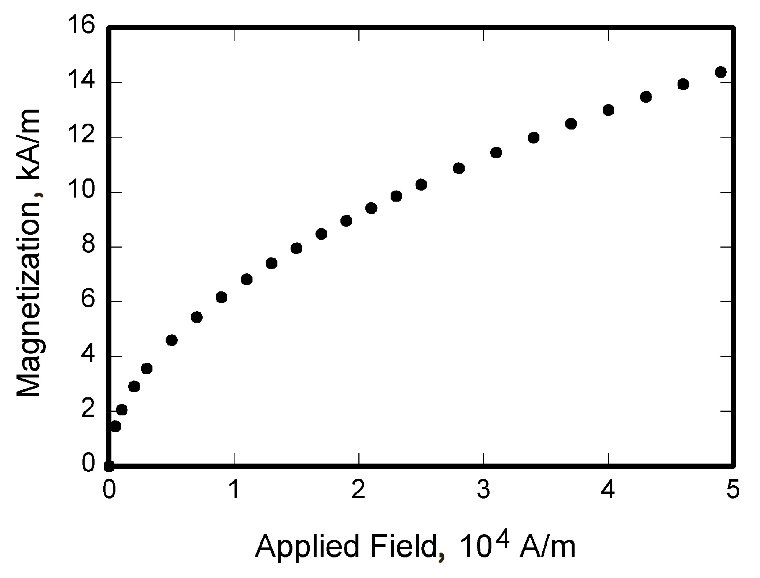
\includegraphics[width=0.4\linewidth]{figures/graph.jpg}
    \caption{Magnetization as a function of applied field}
    \label{fig:sample}
\end{figure}

\subsection{Equations, Numbers, Symbols, and Abbreviations}
Equations are centered and numbered consecutively, with equation numbers in parentheses flush right, as in \autoref{eqn:sample}. Insert a blank line on either side of the equation.
\begin{equation}
    \label{eqn:sample}
    L = C_L \frac{1}{2}\rho V^2 S
\end{equation}

\noindent Be sure that the symbols in your equation are defined before the equation appears, or immediately following. Italicize symbols (T might refer to temperature, but T is the unit tesla). Refer to “Eq. (1),” not “(1)” or “equation (1)” except at the beginning of a sentence: “Equation (1) is…”

Define abbreviations and acronyms the first time they are used in the text, even after they have already been defined in the abstract. Do not use abbreviations in the title.


\section{Results \& Discussion}

In some cases, it might be prefered to split this part into two sections.


\section{Conclusion}
\label{section:conclusion}

\begin{itemize}
	\item First coupling of OpenFAST and preCICE was presented
	\item Coupling with a dummy solver and OpenFOAM was discussed
	\item Although a proof of concept was achieved, some challenging tasks remain to enable a full coupling to CFD solvers
	\item How to map between OpenFAST and an arbitrary CFD solver? Where to place the mapping and smearing algorithm for the ALM method?
	\item This work may serve as a starting point
	\item Has the potential to be developed into a viable open-source alternative for the coupling of OpenFAST to different CFD solvers
\end{itemize}


\section*{Acknowledgments}

Use this section to thank anyone besides the main author(s) who has contributed to the paper. Avoid expressions such as “One of us (S.B.A.) would like to thank…” Instead, write “F. A. Author thanks…”.

%%%%% Bibliography %%%%%

\renewcommand{\bibpreamble}{For a full documentation of the references, please refer to the sample.bib file. You can delete this text/command safely in main.tex at line 73. \cite{example-article,example-article-published-online,example-inbook,example-inbook-series-with-editor,example-inproceedings,example-proceedings,example-report,example-paper,example-phdthesis}}

\bibliography{article}

%%%%% Appendix %%%%%

\section*{Appendix}

An appendix, if needed, should appear at the end of the article.

\end{document}
